\documentclass[12pt, letterpaper, english]{article}
\usepackage[T1]{fontenc}
\usepackage{babel}
\usepackage{amsmath}
\usepackage{amsfonts}
\usepackage{graphicx}
\usepackage{listings}
\lstset{
        language=Verilog,
        tabsize=2,
        breaklines=true,
        numbers=left, 
        numberstyle=\tiny, 
        stepnumber=1, 
        numbersep=5pt,
        basicstyle=\ttfamily,
        framexleftmargin=5mm, 
        frame=single,
        title=morsecode.v,}

\author{
  \textbf{Gramano, Francesco}\\
  \textbf{999203767}\\ %My student number
  \and
  \textbf{Shah, Milind}\\
  \textbf{998907982}\\ %Milo's student number
}
\title{\textbf{CSC258 Final Report:\\ The Morse Code Decoder\\}}
\date{April 5, 2013}
\begin{document}
\maketitle
\section*{Introduction}
\indent\indent We chose to implement a Morse Code Decoder for a few reasons. The first of these reasons was to trace what might now be considered as a primitive beginning to radio communications. We wanted to replicate a self-sufficient version of these means of communication on the DE2 board to revisit the humble beginning of the use of Morse Code as an encoding of the alphabet. More importantly, we wanted to study the ramifications of requiring the synchronization of a finite state machine with the clock of the DE2 board in this process of replicating a Morse Code interpreter.\\
\section*{Methods}
\indent\indent The first problem was to record the duration of a press of $KEY[1]$ on the DE2 board, since the differentiation of a dot ('.') and a dash ('-') in Morse Code is relative to the amount of time that the key is held. Of course, since older standards of Morse Code are much faster than can be provided as input with the press of $KEY[1]$, we used the convention of airway beacons where the shortest unit of time (the dot duration) is $0.5$ seconds. The remaining possible inputs from pressing or the absence of pressing the key are built relatively from the dot duration. So, a dash is interpreted after three dot durations (or $1.5$ seconds), a character break is interpreted after three dot durations of not pressing the key, and a word break (a space between successive characters) is interpreted after seven dot durations (or $3.5$ seconds) of not pressing the key. Then, a character becomes a concatenation of dots and or dashes until either a character break or word break is reached. The duration of the press of $KEY[1]$ was monitored synchronously with the clock by counting the number of cycles that the key had either been pressed or had not been pressed for and computing its duration by dividing the total number of cycles for either by the frequency of the clock of the DE2 board (50 MHz). Since an operator of the Morse Code interpreter could not guarantee that they would, say, hold $KEY[1]$ for exactly $75$ million pulses of the clock in order to register a dot, durations were approximated over a range of time from the exact number, with an allowed error of $0.2$ seconds for each interval. This is reflected in the code in the appendix on lines $114$, $115$, $133$, $134$.\\\\ 
\indent Refer to the following \textit{Huffman Coding} diagram of Morse Code for the representations of letters as sequences of dots and or dashes. Note that a traversal towards the left is equivalent to concatenating a dot to a sequence, a traversal towards the right is equivalent to concatenating a dash to a sequence, and the \textbf{start} state is represented by the empty string which contains no dots or dashes.
\begin{figure}[h!]
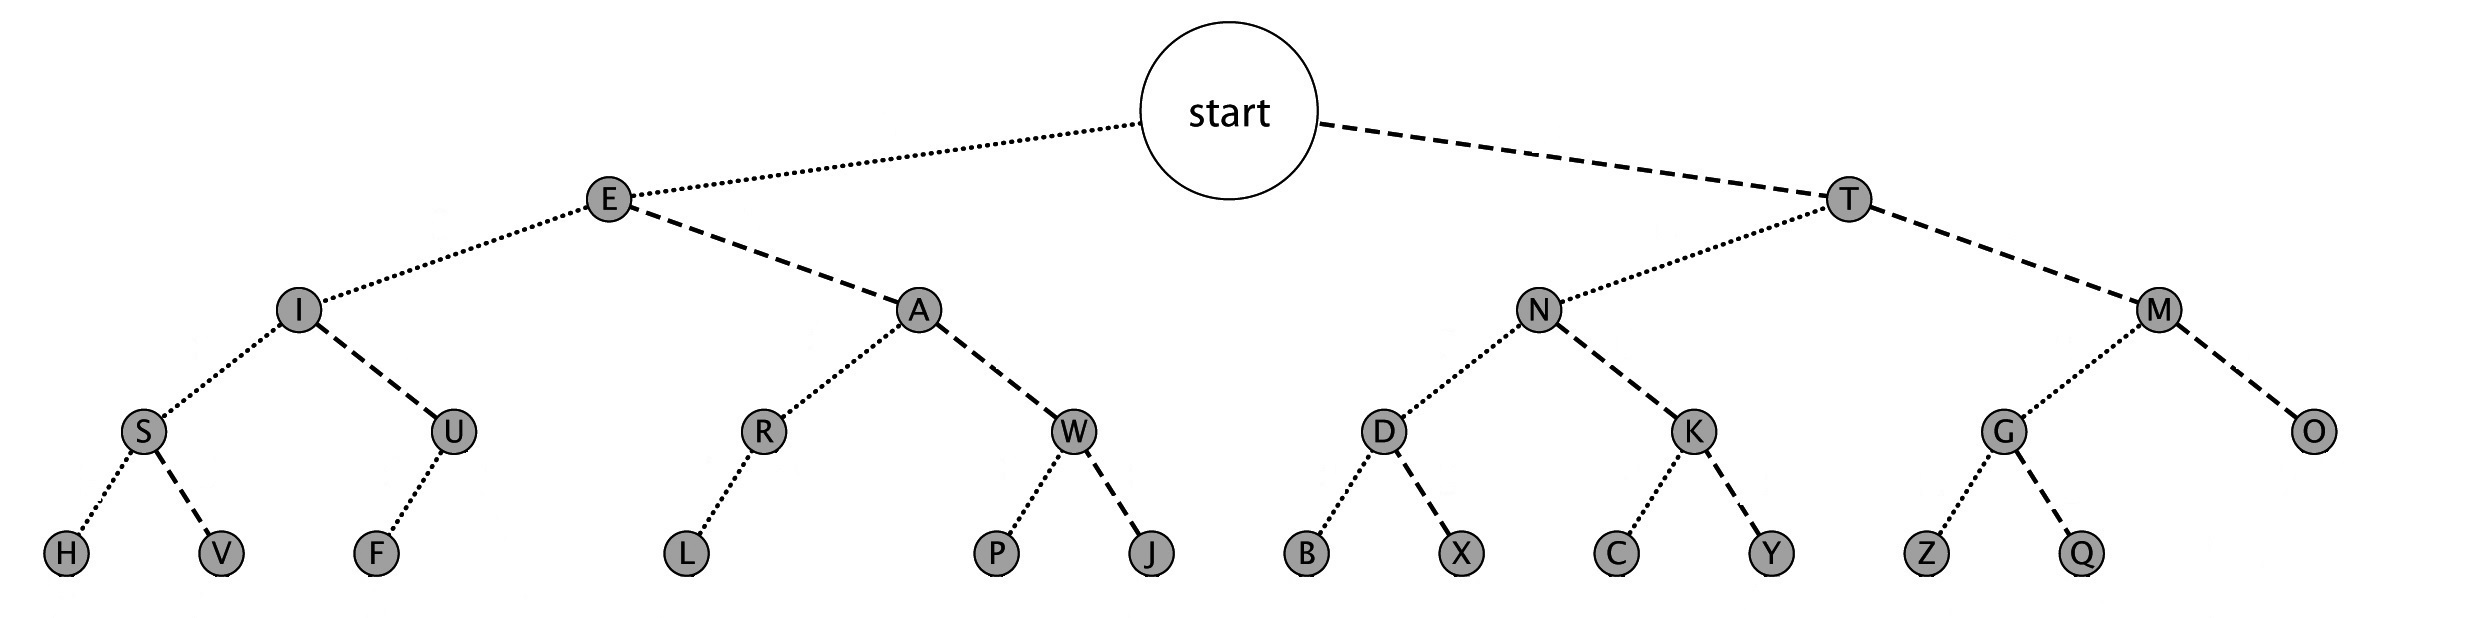
\includegraphics[width = \textwidth]{Tree_Fix.jpg}\caption{A \textit{Huffman Coding} diagram of the representation of Morse Code. \textit{This figure is a simplification of the Huffman Coding diagram for international Morse Code found at http://en.wikipedia.org/wiki/Morse\_code}}
\end{figure}\\\\
\indent In order to restrict the input to the sequences which represent the letters of the alphabet, the characters which have the longest sequence and can therefore not transition to another character (since having the longest sequence would mean that concatenating another dot or dash would result in a non-existent letter) were made to transition to a \textbf{BREAK} state which was also overloaded to represent a character break and a word break.\\ 

\noindent[\textbf{Note:} since a copy of the finite state machine used for transitioning between characters cannot fit between the margins of an 8.5 by 11 inches sheet of paper, the reader will have to interpret the FSM implicitly from \textbf{Figure 1} and the description of the \textbf{BREAK} state. The FSM has 27 states: one for each letter and a \textbf{BREAK} state. A shortened copy of the FSM can still be found in the appendix.]\\\\
\indent After interpreting a word break or a character break, the letter of the alphabet resulting from the cumulated sequence gets printed on the LCD display of the DE2 board and the current display gets shifted over by one character. Effectively, the LCD display acts as a shift register.
\section*{Results}
\indent\indent Overloading the \textbf{BREAK} state turned out to be a greater complication than expected because of the different transitions that could lead to it, and the specific results that should accommodate each of them. Also, designing the FSM turned out to be more difficult than expected because of the large number of cases, each of which must evidently be a correct translation of the previously shown \textit{Huffman Coding} diagram.
\section*{Discussion}
\indent\indent Originally, an attempt was made at simplifying the recording of input by discretizing the moments where the key-press would be monitored. It was initially decided that, with a similar acceptable error of $0.2$ seconds per dot duration, the checking of the key-press would only be monitored at every approximate dot duration. However, since this model would equate three dots with one dash, we eventually realized this would result in an overlap of representations. For example, consider how the letter T is represented by one dash. Discretizing  the checking of input, as was just described, would have it get represented by three consecutive dots, but, this matches the representation of the letter S, so this method of interpretation does not produce unique sequences for characters. That said, we defaulted to counting the number of cycles that $KEY[1]$ would have \textbf{continuously} been held or not been held for. \\\\
\indent Similarly, we initially attempted to enumerate the states that represent the characters as a traversal of the \textit{Huffman Coding} diagram as a binary tree, where a traversal to a left child would concatenate a $0$ and a traversal to a right child would concatenate a $1$. However, since we were only able to store these as binary numbers and not strings, leading zeroes became indistinguishable and state representations were not unique. For example, consider how state $E$ would be enumerated as $0$, and state $I$ would be enumerated as $00$. Treating these representations as numbers, they get treated the same. We solved this problem by enumerating the states by a level-order traversal of the \textit{Huffman Coding} diagram as a binary tree, starting from $1$. With this method, state $E$ was $1$, state $T$ was $2$, and so on and so forth. This is visible towards the beginning of the code in the appendix (on lines $37$ to $43$ of morsecode.v).\\\\
\indent The Morse Code interpreter was mostly functional; however, although the dot duration was set to be $0.5$ seconds, it was still somewhat difficult to hold $KEY[1]$ for the proper durations in order to represent the desired character. This also made it much harder to verify. Though the idea of using a range of time to approximate the durations of each kind of input was practical and helpful, the approximate durations were too small, especially for any beginner of Morse Code.\\\\
\indent We learned that though some of the Morse Code sequences of characters are prefixes of sequences of other characters and monopolizing on this property to create a finite state machine would be elegant, it turns out to be more of a complication. Synchronizing the finite state machine with the LCD display and the clock of the DE2 board becomes a hassle since the transitions of the characters that have the longest accepted sequences (the characters which are represented as leaves on the previous \textit{Huffman Coding} diagram) need to be treated differently from the other characters. This is reflected in the code in the appendix where the reader will see '$\#1000$', which was used at certain points to delay certain transitions of the FSM from executing the remainder of the always block that surrounded it.\\\\
\indent To make it easier for an operator to get used to the device, we would let them specify their average input speed with the switches at execution. With their average speed (in words per minute) we would calculate the dot duration, $T$ (in milliseconds), with the formula $T = \frac{1200}{W}$, where they would be specifying $W$. Approximate ranges surrounding each duration could still be used and the ranges and remaining durations would be calculated relatively from the new dot duration, as per their relative lengths stated earlier.
\section*{Conclusion}
\indent\indent Through the process of constructing the Morse Code interpreter we understood that the simplicity of an earlier version was only meant to be decoded by a human operator; though, using a finite state machine to interpret Morse Code was a good exercise of the use of Verilog and the synchronization to the clock. With the previously noted extension of giving the operator the ability to specify their own input speed, this method of automating the interpretation of Morse Code could be found practical, especially for a beginner who would otherwise have to look up the Morse Code sequence of every character.
\newpage
\part*{Appendix}
The code of the main module:
\begin{lstlisting}
module morsecode(
  input CLOCK_50,    //50 MHz clock
  input [1:0] KEY,    //KEY1 is the morse key
  inout [35:0] GPIO_0,GPIO_1,
  output LCD_ON,
  output LCD_BLON,
  output LCD_RW,
  output LCD_EN,
  output LCD_RS,
  input	PS2_DAT,
  input	PS2_CLK,
  inout [7:0] LCD_DATA,
  output [7:0] LEDG
);

  reg [31:0] CCount; //Clock cycle count
  reg [31:0] Kcount; //Key-press clock cycle count
  reg [31:0] Bcount; //Inactivity clock cycle count
  
  reg w; //w == 1 --> dash, w == 0 --> dot
  reg v; //v == 0 --> c break, v == 1 --> w break
 
  reg newdot; //whether there is a new dot/dash
  reg newbreak; //whether there is a new break
  
  wire reset;
  wire ore;
  reg pulse;
  
  reg [7:0] letter_one; //for immediate letter of the first row
  reg [7:0] letter_two; //for immediate letter of the second row
  reg [127:0] letters_LCD_one; //holds the values of the first row of the LCD
  reg [127:0] letters_LCD_two; //holds the values of the second row of the LCD
	
	//State enumeration for character FSM
	parameter 
	A = 5'd4, B = 5'd21, C = 5'd23, D = 5'd11,
	E = 5'd1, F = 5'd17, G = 5'd13, H = 5'd15,
	I = 5'd3, J = 5'd20, K = 5'd12, L = 5'd18,
	M = 5'd6, N = 5'd5, O = 5'd14, P = 5'd19,
	Q = 5'd26, R = 5'd9, S = 5'd7, T = 5'd2,
	U = 5'd8, V = 5'd16, W = 5'd10, X = 5'd22,
	Y = 5'd24, Z = 5'd25, BREAK = 4'd0;
	
	//The Characters' values for the LCD
	parameter
	LA = 8'h41, LB = 8'h42, LC = 8'h43, LD = 8'h44,
	LE = 8'h45,	LF = 8'h46, LG = 8'h47, LH = 8'h48,
	LI = 8'h49, LJ = 8'h4A, LK = 8'h4B, LL = 8'h4C,
	LM = 8'h4D, LN = 8'h4E, LO = 8'h4F, LP = 8'h50,
	LQ = 8'h51, LR = 8'h52, LS = 8'h53, LT = 8'h54,
	LU = 8'h55, LV = 8'h56, LW = 8'h57, LX = 8'h58,
	LY = 8'h59, LZ = 8'h5A, DOT = 8'h2E, DASH = 8'h2D,
	SPACE = 8'h20; 
  
  reg [4:0] y_Q, Y_D; /* y_Q == current state, 
  Y_D == next state */
  
  //Set defaults
  initial
	begin
	  y_Q = BREAK;
	  Y_D = BREAK;
      letters_LCD_two[7:0] = SPACE;
      letters_LCD_two[15:8] = SPACE;
      letters_LCD_two[23:16] = SPACE;
      letters_LCD_two[31:24] = SPACE;
      letters_LCD_two[39:32] = SPACE;
      letters_LCD_two[47:40] = SPACE;
      letters_LCD_two[55:48] = SPACE;
      letters_LCD_two[63:56] = SPACE;
      letters_LCD_two[71:64] = SPACE;
      letters_LCD_two[79:72] = SPACE;
      letters_LCD_two[87:80] = SPACE;
      letters_LCD_two[95:88] = SPACE;
      letters_LCD_two[103:96] = SPACE;
      letters_LCD_two[111:104] = SPACE;
      letters_LCD_two[119:112] = SPACE;
      letters_LCD_two[127:120] = SPACE;
		
      letters_LCD_one[7:0] = SPACE;
      letters_LCD_one[15:8] = SPACE;
      letters_LCD_one[23:16] = SPACE;
      letters_LCD_one[31:24] = SPACE;
      letters_LCD_one[39:32] = SPACE;
      letters_LCD_one[47:40] = SPACE;
      letters_LCD_one[55:48] = SPACE;
      letters_LCD_one[63:56] = SPACE;
      letters_LCD_one[71:64] = SPACE;
      letters_LCD_one[79:72] = SPACE;
      letters_LCD_one[87:80] = SPACE;
      letters_LCD_one[95:88] = SPACE;
      letters_LCD_one[103:96] = SPACE;
      letters_LCD_one[111:104] = SPACE;
      letters_LCD_one[119:112] = SPACE;
      letters_LCD_one[127:120] = SPACE;
	end
	
  always @ (posedge CLOCK_50) begin
	  if (CCount >= 25000000) begin
			CCount = 0;
			pulse = ~pulse;
	  end else begin
			CCount = CCount + 1;
	  end
	  
	  newbreak = 0;
	  newdot = 0;
	  
	  if (!KEY[1]) begin
			Kcount = Kcount + 1;
			if (Bcount > 0) begin
				if (Bcount > 15000000) begin
					if (Bcount > 91000000) begin
						if (Bcount >= 4294967196) begin
							Bcount = 0; //reset
						end else begin
							v = 1; //word break
							newbreak = 1;
						end
					end else begin
						v = 0; //character break
						newbreak = 1;
					end
				end
			end
			Bcount = 0;
	  end 
	  if (KEY[1]) begin
			Bcount = Bcount + 1;
			if (Kcount > 0) begin
				if (Kcount > 15000000) begin
					if (Kcount > 39000000) begin
						if (Kcount >= 4294967196) begin
							Kcount = 0; //reset 
						end else begin
							w = 1; //dash
							newdot = 1;
						end
					end else begin
						w = 0; //dot
						newdot = 1;
					end
				end
			end
			Kcount = 0;
	  end
  end
	  
  assign LEDG[7:0] = {~pulse,pulse,~pulse,pulse,~pulse,pulse,~pulse,pulse};
  assign ore = newdot ^ newbreak;
  
  
  /* Due to the nature of the previous loop and how
   it affects newdot and newbreak, they will never
    be the same so we can set 
    ore = newdot || newbreak, but it is left as a 
    xor just to be clear that we're avoiding
     unsteady behaviour nonetheless */

always @(posedge ore)	  
  begin: state_table
  case (newdot)
	1: begin
	case (y_Q)
		BREAK: 
			if (w) begin
				Y_D = T;
				letter_two = DASH;
				y_Q = Y_D;
					
				//Shift a dash into the second row
				letters_LCD_two = letters_LCD_two >> 8;
				letters_LCD_two[127:120] = letter_two;
				#1000; //prevent completion of the block 
			end
			else begin
				Y_D = E;
				letter_two = DOT;
				y_Q = Y_D;
					
				//Shift a dot into the second row
				letters_LCD_two = letters_LCD_two >> 8;
				letters_LCD_two[127:120] = letter_two;
				#1000; //prevent completion of the block 
			end
			
		E: 
			if (w) begin
				Y_D = A;
				letter_two = DASH;
				y_Q = Y_D;
				
				//Shift a dash into the second row
				letters_LCD_two = letters_LCD_two >> 8;
				letters_LCD_two[127:120] = letter_two;
				#1000; //prevent completion of the block 
			end
			else begin
				Y_D = I;
				letter_two = DOT;
				y_Q = Y_D;
				
				//Shift a dot into the second row
				letters_LCD_two = letters_LCD_two >> 8;
				letters_LCD_two[127:120] = letter_two;
				#1000; //prevent completion of the block 
			end
			
		T: 
			if (w) begin
				Y_D = M;
				letter_two = DASH;
				y_Q = Y_D;
				
				//Shift a dash into the second row
				letters_LCD_two = letters_LCD_two >> 8;
				letters_LCD_two[127:120] = letter_two;
			end
			else begin
				Y_D = N;
				letter_two = DOT;
				y_Q = Y_D;
				
				//Shift a dot into the second row
				letters_LCD_two = letters_LCD_two >> 8;
				letters_LCD_two[127:120] = letter_two;
				#1000; //prevent completion of the block 
			end
			
		I: 
			if (w) begin
				Y_D = U;
				letter_two = DASH;
				y_Q = Y_D;
				
				//Shift a dash into the second row
				letters_LCD_two = letters_LCD_two >> 8;
				letters_LCD_two[127:120] = letter_two;
				#1000; //prevent completion of the block 
			end
			else begin
				Y_D = S;
				letter_two = DOT;
				y_Q = Y_D;
				
				//Shift a dot into the second row
				letters_LCD_two = letters_LCD_two >> 8;
				letters_LCD_two[127:120] = letter_two;
				#1000; //prevent completion of the block 
			end
			
		A: 
			if (w) begin
				Y_D = W;
				letter_two = DASH;
				y_Q = Y_D;
				
				//Shift a dash into the second row
				letters_LCD_two = letters_LCD_two >> 8;
				letters_LCD_two[127:120] = letter_two;
				#1000; //prevent completion of the block 
			end
			else begin
				Y_D = R;
				letter_two = DOT;
				y_Q = Y_D;
				
				//Shift a dot into the second row
				letters_LCD_two = letters_LCD_two >> 8;
				letters_LCD_two[127:120] = letter_two;
				#1000; //prevent completion of the block 
			end
			
		N: 
			if (w) begin
				Y_D = K;
				letter_two = DASH;
				y_Q = Y_D;
				
				//Shift a dash into the second row
				letters_LCD_two = letters_LCD_two >> 8;
				letters_LCD_two[127:120] = letter_two;
				#1000; //prevent completion of the block 
			end
			else begin
				Y_D = D;
				letter_two = DOT;
				y_Q = Y_D;
				
				//Shift a dot into the second row
				letters_LCD_two = letters_LCD_two >> 8;
				letters_LCD_two[127:120] = letter_two;
				#1000; //prevent completion of the block 
			end
			
		M: 
			if (w) begin
				Y_D = O;
				letter_two = DASH;
				y_Q = Y_D;
				
				//Shift a dash into the second row
				letters_LCD_two = letters_LCD_two >> 8;
				letters_LCD_two[127:120] = letter_two; 
				#1000; //prevent completion of the block
			end
			else begin
				Y_D = G;
				letter_two = DOT;
				y_Q = Y_D;
				
				//Shift a dot into the second row
				letters_LCD_two = letters_LCD_two >> 8;
				letters_LCD_two[127:120] = letter_two;
				#1000; //prevent completion of the block
			end
			
		S: 
			if (w) begin
				Y_D = V;
				letter_one = LV;
				letter_two = DASH;
				y_Q = Y_D;
				
				//Shift a dash into the second row
				letters_LCD_two = letters_LCD_two >> 8;
				letters_LCD_two[127:120] = letter_two;
				#1000; //prevent completion of the block
			end
			else begin
				Y_D = H;
				letter_one = LH;
				letter_two = DOT;
				y_Q = Y_D;
				
				//Shift a dot into the second row
				letters_LCD_two = letters_LCD_two >> 8;
				letters_LCD_two[127:120] = letter_two;  
				#1000; //prevent completion of the block
			end
			
		U: 
			if (!w) begin
				Y_D = F;
				letter_one = LF;
				letter_two = DOT;
				y_Q = Y_D;
				
				//Shift a dot into the second row
				letters_LCD_two = letters_LCD_two >> 8;
				letters_LCD_two[127:120] = letter_two;
			end
			else begin
				Y_D = BREAK;
				letter_one = LU;
				y_Q = Y_D;
				#1000; //prevent completion of the block 
			end
			
		R: 
			if (!w) begin
				Y_D = L;
				letter_one = LL;
				letter_two = DOT;
				y_Q = Y_D;
				
				//Shift a dot into the second row
				letters_LCD_two = letters_LCD_two >> 8;
				letters_LCD_two[127:120] = letter_two;
				#1000; //prevent completion of the block  
			end
			else begin
				Y_D = BREAK;
				letter_one = LR;
				y_Q = Y_D;
			end
			
		W: 
			if (w) begin
				Y_D = J;
				letter_one = LJ;
				letter_two = DASH;
				y_Q = Y_D;
				
				//Shift a dash into the second row
				letters_LCD_two = letters_LCD_two >> 8;
				letters_LCD_two[127:120] = letter_two;
				#1000; //prevent completion of the block 
			end
			else begin
				Y_D = P;
				letter_one = LP;
				letter_two = DOT;
				y_Q = Y_D;
				
				//Shift a dot into the second row
				letters_LCD_two = letters_LCD_two >> 8;
				letters_LCD_two[127:120] = letter_two;
				#1000; //prevent completion of the block
			end
			
		D: 
			if (w) begin
				Y_D = X;
				letter_one = LX;
				letter_two = DASH;
				y_Q = Y_D;
				
				//Shift a dash into the second row
				letters_LCD_two = letters_LCD_two >> 8;
				letters_LCD_two[127:120] = letter_two;
			end
			else begin
				Y_D = B;
				letter_one = LB;
				letter_two = DOT;
				y_Q = Y_D;
				
				//Shift a dot into the second row
				letters_LCD_two = letters_LCD_two >> 8;
				letters_LCD_two[127:120] = letter_two;
			end
			
		K: 
			if (w) begin
				Y_D = Y;
				letter_one = LY;
				letter_two = DASH;
				y_Q = Y_D;
				
				//Shift a dash into the second row
				letters_LCD_two = letters_LCD_two >> 8;
				letters_LCD_two[127:120] = letter_two;
			end
			else begin
				Y_D = C;
				letter_one = LC;
				letter_two = DOT;
				y_Q = Y_D;
				
				//Shift a dot into the second row
				letters_LCD_two = letters_LCD_two >> 8;
				letters_LCD_two[127:120] = letter_two;
			end
			
		G: 
			if (w) begin
				Y_D = Q;
				letter_one = LQ;
				letter_two = DASH;
				y_Q = Y_D;
				
				//Shift a dash into the second row
				letters_LCD_two = letters_LCD_two >> 8;
				letters_LCD_two[127:120] = letter_two;
			end
			else begin
				Y_D = Z;
				letter_one = LZ;
				letter_two = DOT;
				y_Q = Y_D;
				
				//Shift a dot into the second row
				letters_LCD_two = letters_LCD_two >> 8;
				letters_LCD_two[127:120] = letter_two;
				end
		default: Y_D = BREAK;
	endcase
	end
	
	/* newbreak == 1 since ore == newbreak ^ newdot 
	and newdot is false */
	0: case (v)
		0: 
			begin
				Y_D = BREAK;
				case (y_Q)
					E: letter_one = LE;
					T: letter_one = LT;
					I: letter_one = LI;
					A: letter_one = LA;
					N: letter_one = LN;
					M: letter_one = LM;
					S: letter_one = LS;
					U: letter_one = LU;
					R: letter_one = LR;
					W: letter_one = LW;
					D: letter_one = LD;
					K: letter_one = LK;
					G: letter_one = LG;
					O: letter_one = LO;
					H: letter_one = LH;
					V: letter_one = LV;
					F: letter_one = LF;
					L: letter_one = LL;
					P: letter_one = LP;
					J: letter_one = LJ;
					B: letter_one = LB;
					X: letter_one = LX;
					C: letter_one = LC;
					Y: letter_one = LY;
					Z: letter_one = LZ;
					Q: letter_one = LQ;

				endcase
				y_Q = Y_D;
				//Shift letter's value into the register
				letters_LCD_one = letters_LCD_one >> 8;
				letters_LCD_one[127:120] = letter_one;
				#1000; //prevent completion of the block
			end
			
		1: 
			begin
				letter_one = SPACE;
				letter_two = SPACE;
				Y_D = BREAK;
				y_Q = Y_D;
				
				//Shift letter's value into the register
				letters_LCD_one = letters_LCD_one >> 8;
				letters_LCD_one[127:120] = letter_one;
				letters_LCD_two = letters_LCD_two >> 8;
				letters_LCD_two[127:120] = letter_two;
				#1000; //prevent completion of the block
			end
		endcase
	endcase 
  end // state_table
	
	//Display the two rows
	LCD disp (CLOCK_50, KEY[1:0], GPIO_0, GPIO_1, LCD_ON, LCD_BLON, LCD_RW, LCD_EN,
	LCD_RS, PS2_DAT, PS2_CLK, LCD_DATA, letters_LCD_one, letters_LCD_two);
endmodule


\end{lstlisting}
The module named $LCD$ which is referred to in the code above is a slight modification of a previously used 'lcdlab' which can be found at\\ http://www.johnloomis.org/digitallab/lcdlab/lcdlab3/lcdlab3.html\\\\
The modification simply allowed the module to display the registries that stored the values of both rows of the LCD.\newpage
\noindent A portion of the FSM used for the transition of characters. There are $27$ states: one for each letter and one for the \textbf{BREAK} state.
\begin{center}
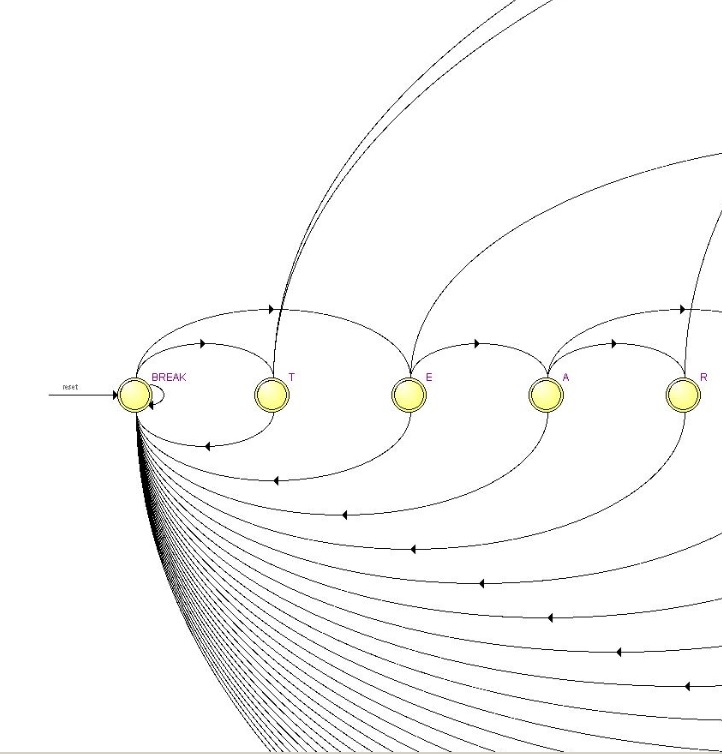
\includegraphics[scale=0.85]{Short.jpg}
\end{center}
\end{document}
%\begin{lstlisting}
%module
%\end{lstlisting}